\section{Approach}

I developed a two-stage approach to the \gls{srm} design problem.
The first stage is a 1D quasi-steady rocket optimization model,
which determines both the internal flow quantities and a basic description
of the internal geometry. The model takes the following inputs:
\begin{itemize}
    \item Coarse time and spatial discretization of the rocket sections
    \item The desired thrust profile of the rocket
    \item Bounds on the rocket external dimensions, if desired
    \item Material properties of the propellant
\end{itemize}

\tdplotsetmaincoords{50}{130}
\tdplotsetrotatedcoords{0}{90}{0}

\begin{figure}
    \begin{center}
        \begin{tikzpicture}[tdplot_main_coords]
            \draw[thick,->] (0,0,0) -- (1,0,0) node[anchor=north east]{$l$};
            \draw[thick,->] (0,0,0) -- (0,-1,0) node[anchor=south west]{$r$};
            \draw[thick,dashed] (0,0,0) -- (-4,0,0) node[anchor=north west]{$$};
            % Blue circles
            \tdplotdrawarc[tdplot_rotated_coords, color=blue]{(0,0,-4)}{2}{0}{360}{anchor=south west}{$\pi r^2$};
            \tdplotdrawarc[tdplot_rotated_coords, color=blue]{(0,0,0)}{2}{0}{360}{anchor=south west}{$$};
            % Blue dashed lines
            \draw[thick,dashed,color=blue] (0,-1.414,1.414) -- (-4,-1.414,1.414) node[anchor=south east]{$l_{\rm{sec}}$};
            \draw[thick,dashed,color=blue] (0,1.414,-1.414) -- (-4,1.414,-1.414) node[anchor=north west]{$l_{\rm{sec}}$};

            % Tophalf, top circle
            \tdplotdrawarc[tdplot_rotated_coords, color=red]{(-0.25,0.25,-4)}{1}{25}{248}{anchor=north west}{$$};
            % Top half, bottom circle
            \tdplotdrawarc[tdplot_rotated_coords, color=red]{(0.25,-0.25,-4)}{1}{205}{428}{anchor=north west, right=0.5cm, above=0.5cm}{$A_{in}$};
            % Bottom half, top circle
            \tdplotdrawarc[tdplot_rotated_coords, color=red]{(-0.25,0.25,0)}{1.25}{28}{243}{anchor=north west}{$$};
            % Bottom half, bottom circle
            \tdplotdrawarc[tdplot_rotated_coords, color=red]{(0.25,-0.25,0)}{1.25}{208}{425}{anchor=north west, right=0.5cm}{$A_{out}$};

            % Red dashed lines
            \draw[thick,dashed,color=red] (0,-0.85,0.85) -- (-4,-0.67,0.67) node[anchor=south east]{$$};
            \draw[thick,dashed,color=red] (0,0.85,-0.85) -- (-4,0.67,-0.67) node[anchor=north west]{$$};
        \end{tikzpicture}
    \end{center}
    \caption{Labeling of a single section of the rocket. }
    \label{fig:SRMsection}
\end{figure}

The optimization model, which is a signomial (i.e. difference-of-log-convex) program, determines the
flow properties inside and thrust generated by a rocket that has
been partitioned into $n_x$ of sections that evolve in $n_t$ time steps.
I don't want to bore you with the details, but this was possible by performing a
relaxation on all three conservation laws (mass, momentum and energy),
and writing the 1D finite volume approximation of the reactive flow problem
as a signomial program in GPkit\footnote{GPkit is an open-source modeling framework
that abstracts away solvers, and facilitates the use of geometric and signomial programs in engineering design.}.
Figure~\ref{fig:SRMsection} shows a potential cross-section of such a \gls{srm}.
The physical model assumes quasi-steady flow during each timestep, where the fluid travels strictly
in the $l$ direction down the bore drawn in red, and the conservation laws are enforced at
each bore cross-sectional area $A$. The output variables of this model are:
\begin{itemize}
    \item The material properties of the fuel burned in a given section in one time step, which are:
    \begin{itemize}
        \item Porosity of fuel
        \item Mass fraction of propellant
        \item Mass fraction of accelerant
        \item Mass fraction of filler
    \end{itemize}
    \item The arc lengths of shapes of $A_{in}$ and $A_{out}$
    \item The cross-sectional areas of $A_{in}$ and $A_{out}$
\end{itemize}

The idea is to take these output variables, and map them onto a series of
non-intersecting univariate polynomials $p_{i,t}(\theta), i = [1,2,...,n_x], t = [1,...,n_t]$
which describe the internal geometry of the rocket.
Another idea was to map to the bivariate polynomial $p_i(\theta,t)$
which has the requirement to be monotonically increasing in $t$
but I stuck to univariate polynomials since the problem
was difficult enough.
To give context about the kinds of cross-sectional shapes that are currently used in rocket design,
see Figure~\ref{fig:potentialShapes}. The sky really is the limit.
The hope is that this problem has a \gls{sdp} relaxation that can find
polynomials that can fulfill the constraints, at a minimum in a least-squares sense,
since feasibility is not guaranteed.

\begin{figure}[h]
    \begin{center}
        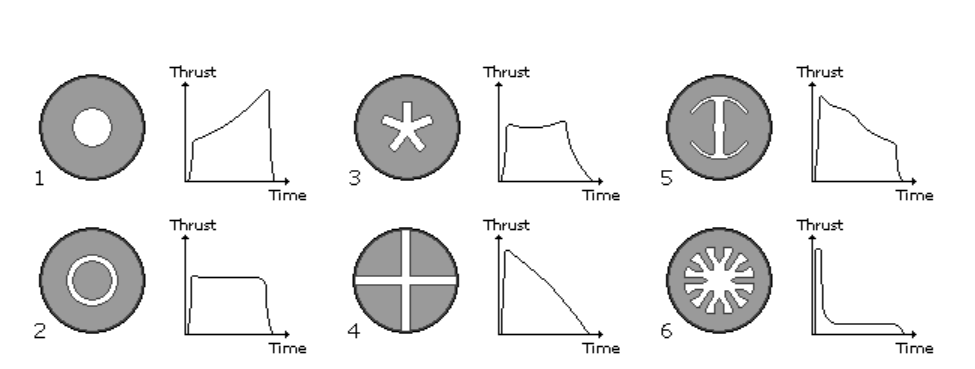
\includegraphics[width=0.7\linewidth]{figures/potentialShapes.PNG}
        \caption{Different thrust profiles may result in very different potential internal configurations of the rocket.
        Image courtesy of Robert A. Braeunig.}
        \label{fig:potentialShapes}
    \end{center}
\end{figure}
